\documentclass{article}
\usepackage{graphicx} % Required for inserting images
\usepackage{subcaption}
\usepackage{xcolor}
\usepackage[paper=a4paper,dvips,top=1.5cm,left=1.5cm,right=1.5cm,
    foot=1cm,bottom=1.5cm]{geometry}
\usepackage{minted}

\title{Embedded Intelligence Lab 1}
\author{Irene Merino Balaguer\\Jonathan Lundström }
\date{\today}

\newcommand{\fig}[3] {
\begin{figure}[H]
\centering
\includegraphics[width=0.5\textwidth]{img/#1/#2.png}
\caption{#3}
\label{figure:#1_#2}
\end{figure}
}

\begin{document}

\maketitle

\section{Task 1 - Exploratory Data Analysis}

\subsection {White Noise Series}
\subsubsection{ Generate a white noise series with N data points (e.g. N can be 100, 1000, 5000,
 or 10000). Then find its actual mean, standard deviation, and draw its line plot,
 histogram, density plot, box plot, lag-1 plot, ACF and PACF graphs (lags up to
 40).}
 With the following given code:
 
\begin{listing}[!ht]
\begin{minted}{python}
seed = 1
rng = numpy.random.default_rng(seed)
c = 1 # Noise Strength
samples = 1000
test_size = 0.20

x = numpy.arange(0, 5, 1/samples)
y_ground_truth = numpy.zeros(x.shape)
y = y_ground_truth + c * rng.normal(0, 1, x.shape)
\end{minted}
\caption{White Noise Generator}
\label{listing:gen_wn}
\end{listing}
We can easily generate a white noise series, then, with the functions provided by the packages matplotlib and statsmodels we can generate the requested graphs. 
\begin{figure}[htbp]
  \centering
  \begin{subfigure}[b]{0.45\textwidth}
    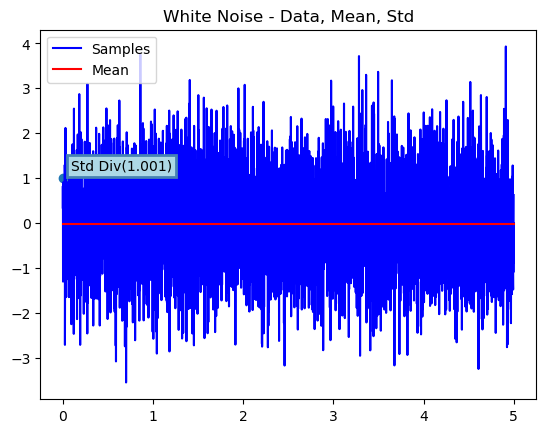
\includegraphics[width=\textwidth]{img/white_noise/data.png}
    \caption{White Noise Generator Data}
    \label{fig:Whitenoiselines}
  \end{subfigure}
  \hfill
  \begin{subfigure}[b]{0.45\textwidth}
    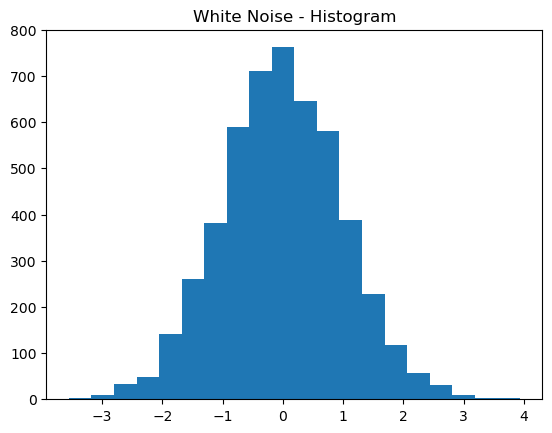
\includegraphics[width=\textwidth]{img/white_noise/histogram.png}
    \caption{White Noise Histogram (20 Buckets)}
    \label{fig:whitenoisehist}
  \end{subfigure}
  \caption{Line and Histogram Plots}
  \label{fig:whitenoise1}
\end{figure}
\begin{figure}[htbp]
  \centering
  \begin{subfigure}[b]{0.45\textwidth}
    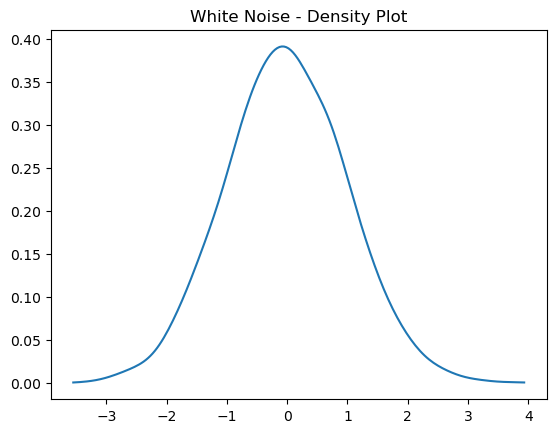
\includegraphics[width=\textwidth]{img/white_noise/density_plot.png}
    \caption{White Noise Density Plot}
    \label{fig:whitenoisedensity}
  \end{subfigure}
  \hfill
  \begin{subfigure}[b]{0.45\textwidth}
    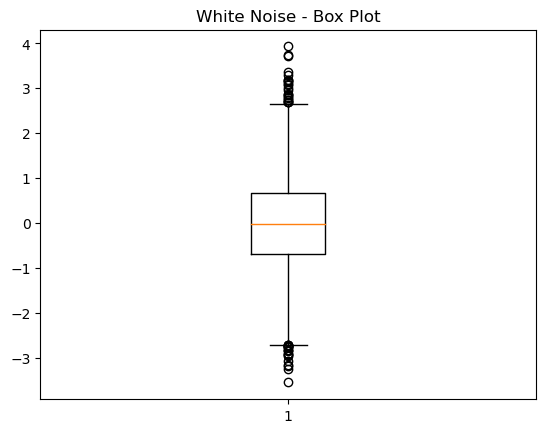
\includegraphics[width=\textwidth]{img/white_noise/box_plot.png}
    \caption{White Noise Box Plot}
    \label{fig:whitenoisebox}
  \end{subfigure}
  \caption{Density and Box Plot}
  \label{fig:whitenoise2}
\end{figure}
\begin{figure}[htbp]
  \centering
  \begin{subfigure}[b]{0.45\textwidth}
    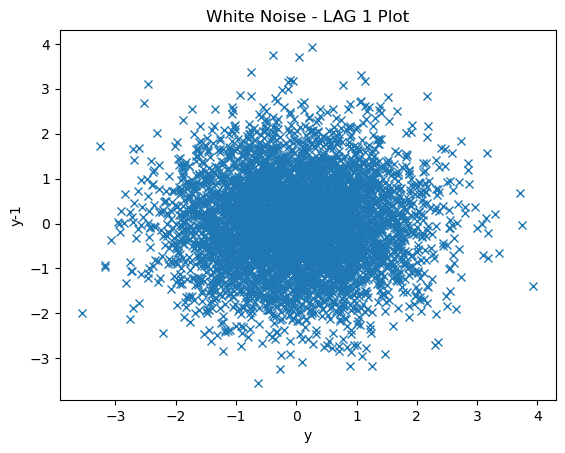
\includegraphics[width=\textwidth]{img/white_noise/lag_1.png}
    \caption{White Noise Lag$_1$}
    \label{fig:whitenoiselag}
  \end{subfigure}
  \hfill
  \begin{subfigure}[b]{0.45\textwidth}
    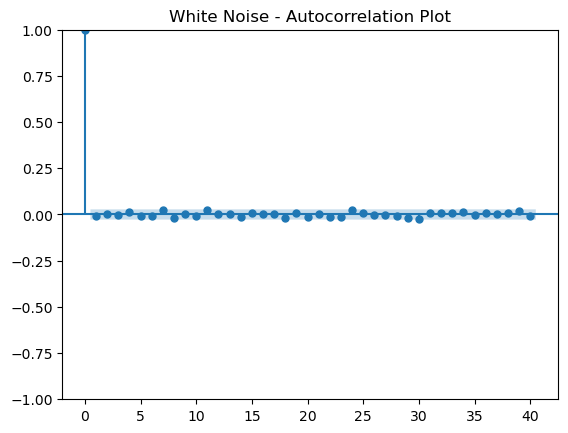
\includegraphics[width=\textwidth]{img/white_noise/acf.png}
    \caption{White Noise ACF}
    \label{fig:whitenoiseacf}
  \end{subfigure}
  \caption{Lag and ACF plots}
  \label{fig:whitenoise3}
\end{figure}
\fig{white_noise}{pacf}{White Noise PACF}
\subsubsection{Generate 100 random series with length 1000 data points, then use the average
 values at each time to produce an average value series. Then repeat the same
 process above.}
 By using the given code we generate 100 random white noise series, then we compute the average of each value.
 \begin{listing}[!ht]
\begin{minted}{python}
for i in x:
    data = c * rng.normal(0, 1, 1000)
    y.append(numpy.average(data))
\end{minted}
\caption{Average Value Series Generator}
\label{listing:gen_wn}
\end{listing}
 Finally, with the same functions as before we obtain the following plots.
 \begin{figure}[htbp]
  \centering
  \begin{subfigure}[b]{0.45\textwidth}
    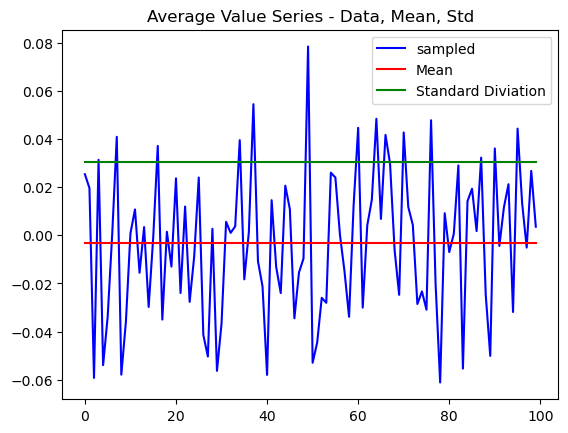
\includegraphics[width=\textwidth]{img/wn_average_value/data.png}
    \caption{White Noise Average Value Generator Data}
    \label{fig:Avgvaluelines}
  \end{subfigure}
  \hfill
  \begin{subfigure}[b]{0.45\textwidth}
    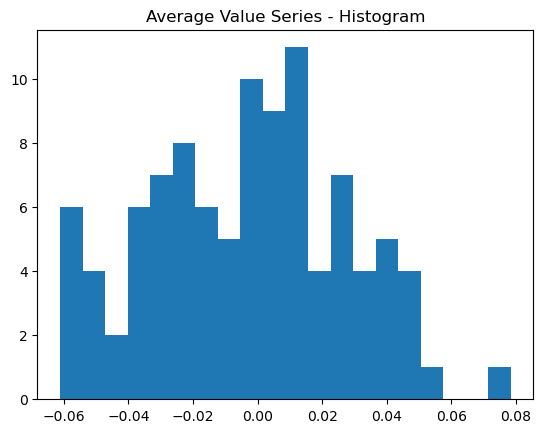
\includegraphics[width=\textwidth]{img/wn_average_value/histogram.png}
    \caption{White Noise Average Value Histogram (20 Buckets)}
    \label{fig:Avgvaluehist}
  \end{subfigure}
  \caption{Line and Histogram Plots}
  \label{fig:avgvalue1}
\end{figure}
\begin{figure}[htbp]
  \centering
  \begin{subfigure}[b]{0.45\textwidth}
    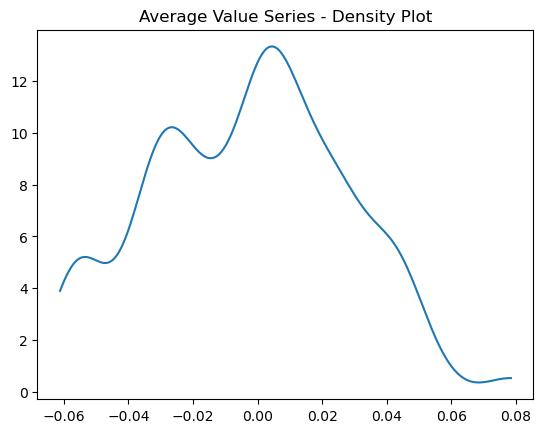
\includegraphics[width=\textwidth]{img/wn_average_value/density_plot.png}
    \caption{White Noise Average Value Density Plot}
    \label{fig:avgvalueedensity}
  \end{subfigure}
  \hfill
  \begin{subfigure}[b]{0.45\textwidth}
    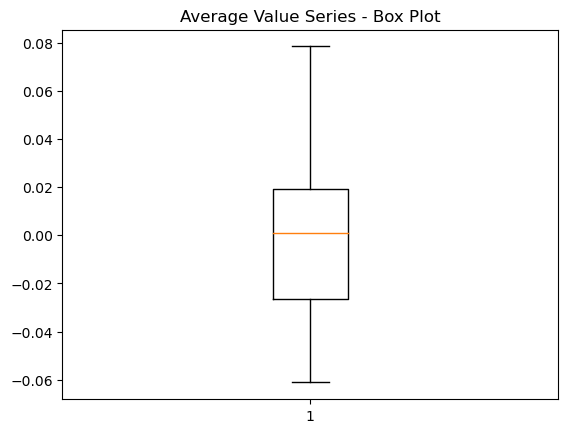
\includegraphics[width=\textwidth]{img/wn_average_value/box_plot.png}
    \caption{White Noise Average Value Box Plot}
    \label{fig:avgvaluebox}
  \end{subfigure}
  \caption{Density and Box Plot}
  \label{fig:avgvalue2}
\end{figure}
\begin{figure}[htbp]
  \centering
  \begin{subfigure}[b]{0.45\textwidth}
    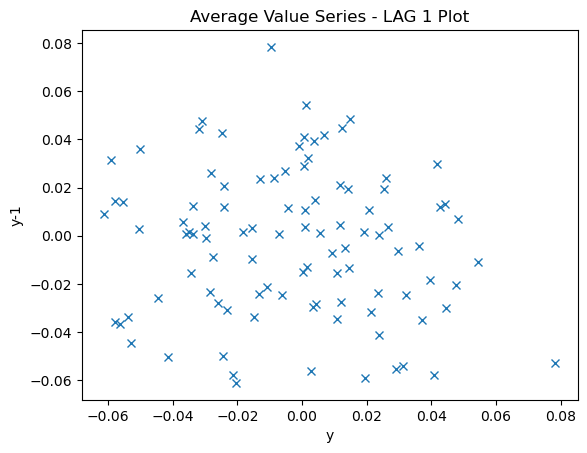
\includegraphics[width=\textwidth]{img/wn_average_value/lag_1.png}
    \caption{White Noise Average Value Lag$_1$}
    \label{fig:avgvaluelag}
  \end{subfigure}
  \hfill
  \begin{subfigure}[b]{0.45\textwidth}
    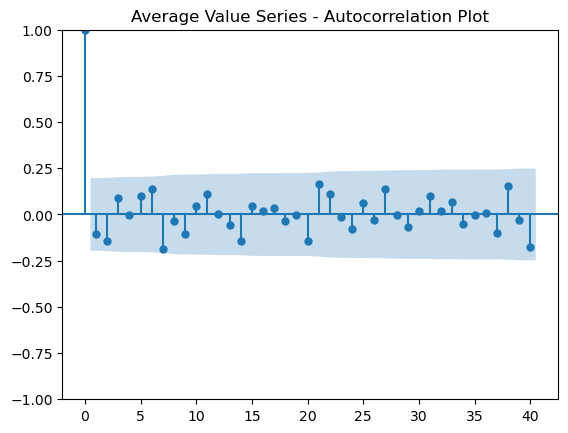
\includegraphics[width=\textwidth]{img/wn_average_value/acf.png}
    \caption{White Noise Average Value ACF}
    \label{fig:avgvalueacf}
  \end{subfigure}
  \caption{Lag and ACF plots}
  \label{fig:whitenoise3}
\end{figure}
\fig{wn_average_value}{pacf}{WN Avg Value PACF}
\subsubsection{Perform randomness test on the white noise series using the Ljung-Box test.}

In the case of the single white noise series Ljung-Box Test resulted in a lb\_pvalue of 0.927168 which is greater then 0.05 meaning the series is random. And for the second case, Ljung-Box Test resulted in a lb\_pvalue of 0.400553 which is greater then 0.05 meaning the series is also random.

\subsubsection{Perform stationarity test on the white noise series using the Augmented Dickey
Fuller (ADF) test.}
In the first case, for the Augmented Dickey Fuller (ADF) test with a max lag of 40 the ADF statistic was -71 with the critical values being -3.43, -2.86, -2.56. With the ADF statistic being smaller then the critical values we can reject the null hypothesis of the data not being stationary. Which agrees with the p\_value of 0.0 which is less then 0.05. So the data is stationary. And in the average value series case for the Augmented Dickey Fuller (ADF) test with a max lag of 40 the ADF statistic was -3.607 with the critical values being -3.504, -2.89, -2.584. With the ADF statistic being smaller then the critical values we can reject the null hypothesis of the data not being stationary. Which agrees with the p\_value of 0.0 056 which is less then 0.05. So the data is stationary.

\subsection{Task 1.2 Random-walk series}
\subsubsection{Realize a simple random walk series with N data points (e.g. N can be 100, 1000,
 5000, or 10000) starting from an initial value of 0 (y0 = 0), and xt = +1,−1.}
 The random walk series can be generated with the following code:
 
\begin{listing}[!ht]
\begin{minted}{python}
N = 1000
x = numpy.arange(0,N)
y = rng.choice([1,-1], x.shape)
y[0] = 0
y = numpy.cumsum(y)
\end{minted}
\caption{Random Walk Series Generator}
\label{listing:gen_random}
\end{listing}

\subsubsection{Then find its actual mean, standard deviation, and draw its line plot, histogram,
 density plot, box plot, lag-1 plot, ACF and PACF graphs (lags up to 40).}

The procedure to get the mean, standard deviation and the plots is the same as in the previous section.
 \begin{figure}[htbp]
  \centering
  \begin{subfigure}[b]{0.45\textwidth}
    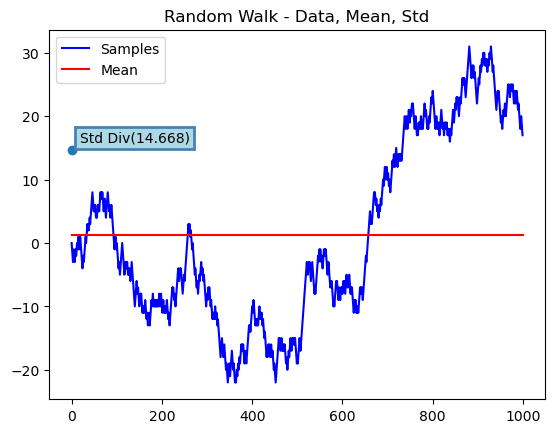
\includegraphics[width=\textwidth]{img/random_walk/data.png}
    \caption{Random Walk Generator Data}
    \label{fig:rndmwalklines}
  \end{subfigure}
  \hfill
  \begin{subfigure}[b]{0.45\textwidth}
    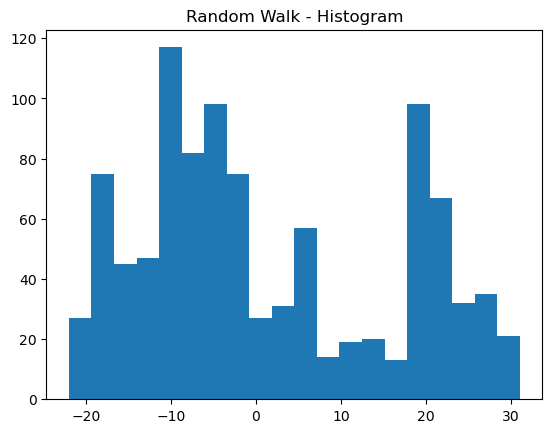
\includegraphics[width=\textwidth]{img/random_walk/histogram.png}
    \caption{Random Walk Histogram (20 Buckets)}
    \label{fig:Rndmwalkhist}
  \end{subfigure}
  \caption{Line and Histogram Plots}
  \label{fig:randomwalk1}
\end{figure}
\begin{figure}[htbp]
  \centering
  \begin{subfigure}[b]{0.45\textwidth}
    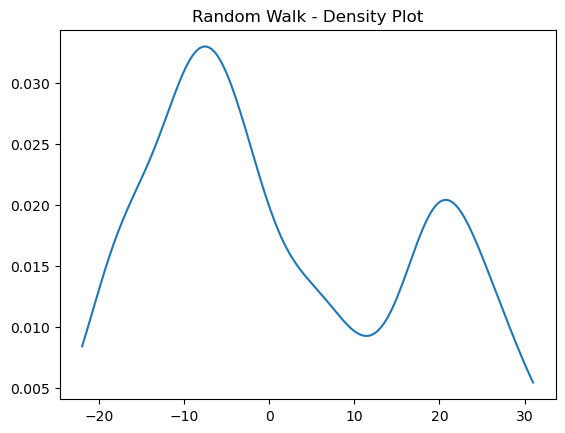
\includegraphics[width=\textwidth]{img/random_walk/density_plot.png}
    \caption{Random Walk Density Plot}
    \label{fig:rndmwalkdensity}
  \end{subfigure}
  \hfill
  \begin{subfigure}[b]{0.45\textwidth}
    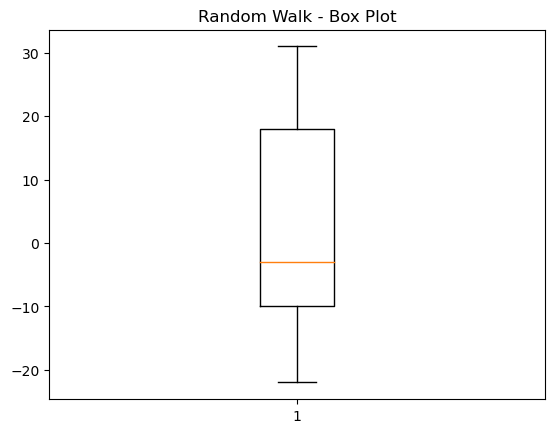
\includegraphics[width=\textwidth]{img/random_walk/box_plot.png}
    \caption{Random Walk Box Plot}
    \label{fig:rndmwalkbox}
  \end{subfigure}
  \caption{Density and Box Plot}
  \label{fig:rndmwalk2}
\end{figure}
\begin{figure}[htbp]
  \centering
  \begin{subfigure}[b]{0.45\textwidth}
    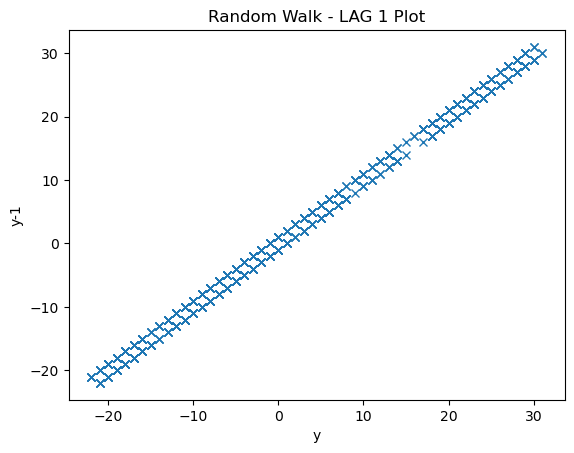
\includegraphics[width=\textwidth]{img/random_walk/lag_1.png}
    \caption{Random Walk Lag$_1$}
    \label{fig:rndmwalklag}
  \end{subfigure}
  \hfill
  \begin{subfigure}[b]{0.45\textwidth}
    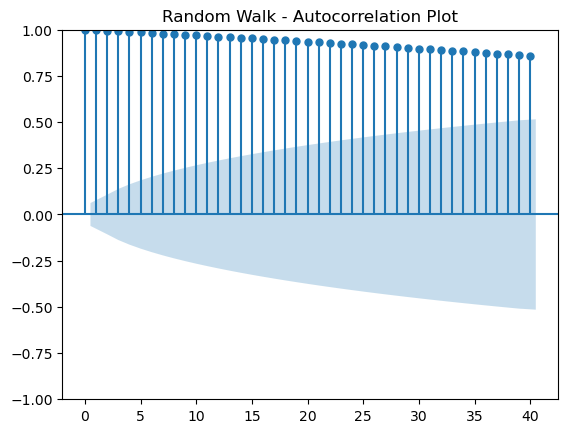
\includegraphics[width=\textwidth]{img/random_walk/acf.png}
    \caption{Random Walk ACF}
    \label{fig:rndmwalkacf}
  \end{subfigure}
  \caption{Lag and ACF plots}
  \label{fig:rndmwalk3}
\end{figure}
\fig{random_walk}{pacf}{Random Walk PACF}

\subsubsection{Perform randomness test on the random walk series using the Ljung-Box test.}

Ljung-Box Test resulted in a lb\_pvalue of 0.0 which is less then 0.05 meaning the series is not random.
\subsubsection{Perform stationarity test on the random walk series using the Augmented Dickey
Fuller (ADF) test. Is the series stationary? If not, which operation can be applied
 to make it stationary?}
 
For the Augmented Dickey Fuller (ADF) test with a max lag of 40 the ADF statistic was -0.813 with the critical values being -3.43, -2.86, -2.56. With the ADF statistic being larger then the critical values we can accept the null hypothesis that the data is not stationary. Which agrees with the p\_value of 0.815 which is greater then 0.05. So the data is not stationary.

One way to make the data stationary is taking the first order derivative this will result in a plot of the choices taken which can be -1 or 1.
\subsubsection*{Answer the following questions:}
\begin{itemize}
    \item \textbf{What methods can be used to check if a series is random? Describe both visualization and statistic test methods.}
\end{itemize}
We have used 1 statistical method to determine a confidence level of randomness called the Ljung-Box test. This test calculates a correlation with various lags to generate a confidence value in the likelyhood of data being random.
For the visual methods lags can be used to show correlation if a trend can be visually observed between data points. An alternative plot would be an autocorrelation plot or partial autocorrelation plot. These can show the seasonality of data and repeatability that can be combined with a threshold. Histograms can also provide insight to data uniformity.
\begin{itemize}
    \item \textbf{What methods can be used to check if a series is stationary? Describe both visualization and statistic test methods.}
\end{itemize}

The Augmented Dickey Fuller test is used to verify stationarity.
The data plot along with mean and standard deviations with a sliding window
\begin{itemize}
    \item \textbf{Why is white noise important for time-series predictions?}
\end{itemize}

When building a model the left over data should be white noise, the reasoning is if the left over data has structure there is room to improve the model.
\begin{itemize}
    \item \textbf{What is the difference between a white noise series and a random walk series?}
\end{itemize}

White noise has a mean of 0, the max values are bounded, and values are independent. A random walk is dependent on the past values so has a strong correlation to $t_{n-1}$.
\begin{itemize}
    \item \textbf{Is it possible to change a random walk series into a series without correlation across its values ? If so, how? Explain also why it can.}
\end{itemize}

The core concept of a random walk is that it correlates to the previous value. but a representation of the series could be constructed by generating a fist order derivative which would result in values that do not correlate due to changes being independently generated.


\subsection{Task 1.3 Global land temperature anomalies series}
\subsubsection{ Use the global land temperature anomalies data to draw line plot, histogram, density
 plot, box-plot, heatmap, lag-1 plot, auto-correlation function (acf) and partial acf
 (pacf) graphs (lags up to 40).}
We extract the data from the provided excel files and draw the plots for the exploratory data analysis.
 \begin{figure}[H]
  \centering
  \begin{subfigure}[b]{0.45\textwidth}
    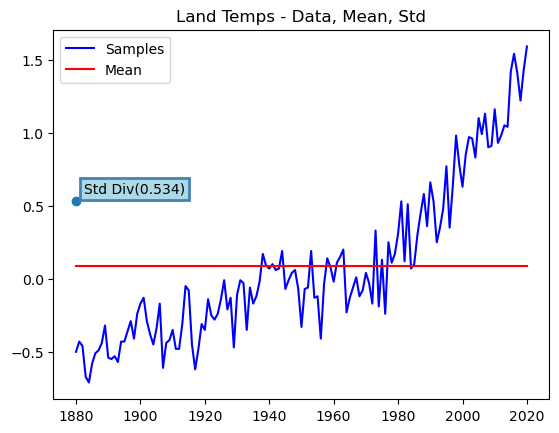
\includegraphics[width=\textwidth]{img/global_temp/data.png}
    \caption{Global Temp Data}
    \label{fig:global_templines}
  \end{subfigure}
  \hfill
  \begin{subfigure}[b]{0.45\textwidth}
    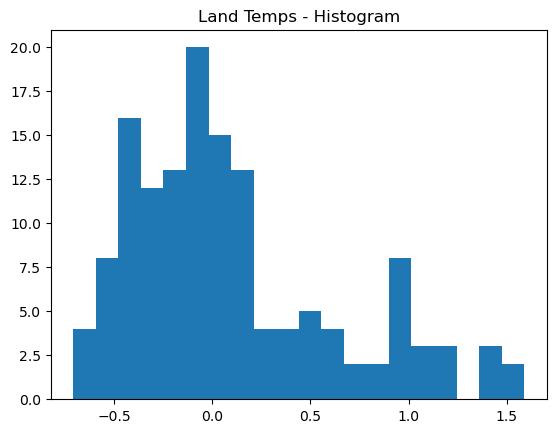
\includegraphics[width=\textwidth]{img/global_temp/histogram.png}
    \caption{Global Temp Histogram (20 Buckets)}
    \label{fig:global_temphist}
  \end{subfigure}
  \caption{Line and Histogram Plots}
  \label{fig:global_temp1}
\end{figure}
\begin{figure}[H]
  \centering
  \begin{subfigure}[b]{0.45\textwidth}
    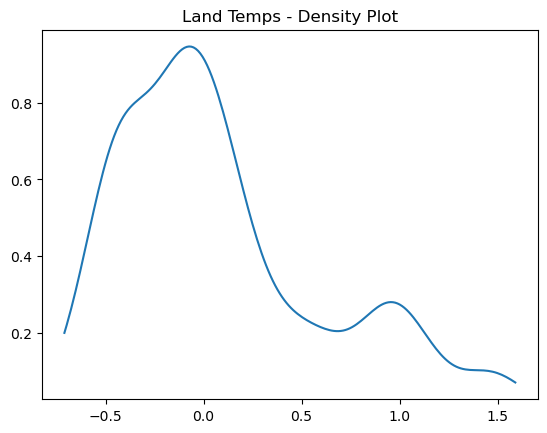
\includegraphics[width=\textwidth]{img/global_temp/density_plot.png}
    \caption{Global Temp Density Plot}
    \label{fig:global_tempdensity}
  \end{subfigure}
  \hfill
  \begin{subfigure}[b]{0.45\textwidth}
    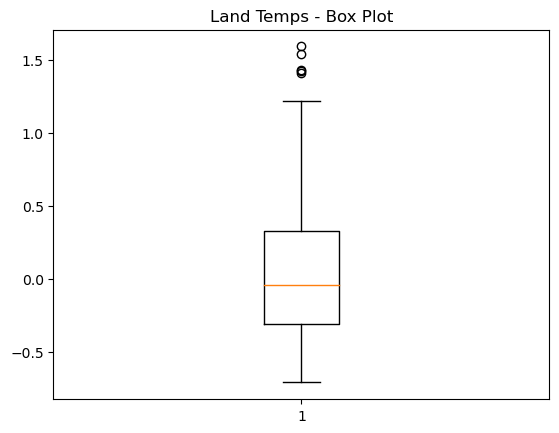
\includegraphics[width=\textwidth]{img/global_temp/box_plot.png}
    \caption{Global Temp Box Plot}
    \label{fig:global_tempbox}
  \end{subfigure}
  \caption{Density and Box Plot}
  \label{fig:global_temp2}
\end{figure}
\begin{figure}[H]
  \centering
  \begin{subfigure}[b]{0.45\textwidth}
    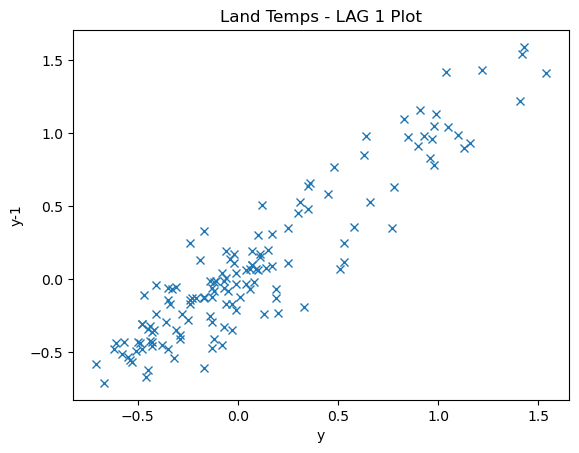
\includegraphics[width=\textwidth]{img/global_temp/lag_1.png}
    \caption{Global Temp Lag$_1$}
    \label{fig:global_templag}
  \end{subfigure}
  \hfill
  \begin{subfigure}[b]{0.45\textwidth}
    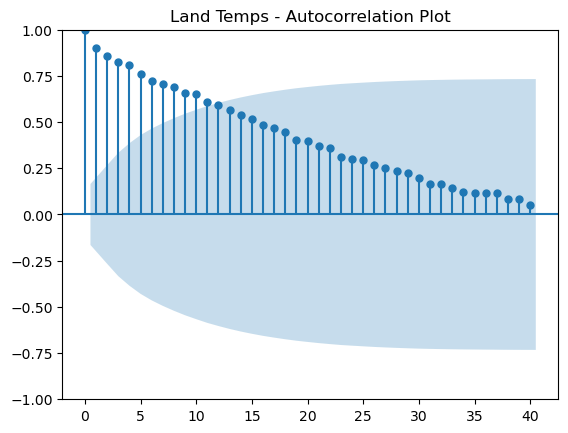
\includegraphics[width=\textwidth]{img/global_temp/acf.png}
    \caption{Global Temp ACF}
    \label{fig:global_tempacf}
  \end{subfigure}
  \caption{Lag and ACF plots}
  \label{fig:global_temp3}
\end{figure}
\begin{figure}[htbp]
  \centering
  \begin{subfigure}[b]{0.45\textwidth}
    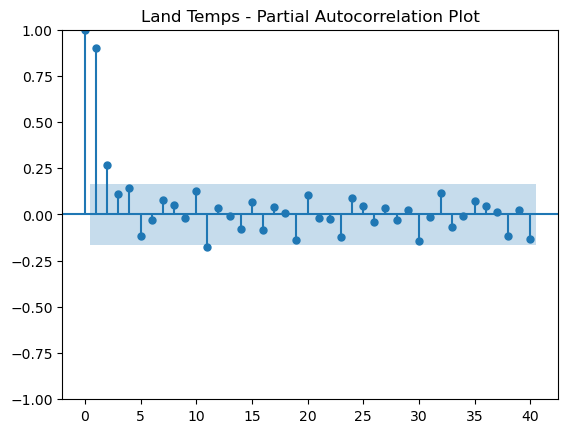
\includegraphics[width=\textwidth]{img/global_temp/pacf.png}
    \caption{Global Temp PACF}
    \label{fig:global_pacf}
  \end{subfigure}
  \hfill
  \begin{subfigure}[b]{0.45\textwidth}
    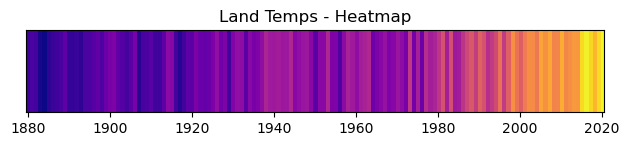
\includegraphics[width=\textwidth]{img/global_temp/heatmap.png}
    \caption{Global Temp Heatmap}
    \label{fig:global_heatmap}
  \end{subfigure}
  \caption{PACF and Heatmap}
  \label{fig:global_temp4}
\end{figure}

\subsubsection{Take the first order difference of the temperature anomaly dataset. Draw line plot,
 histogram, density plot, box-plot, heatmap, lag-1 plot, acf and pacf graphs (lags up
 to 40).}

 We compute the first order difference of the previous dataset with the following code:
\begin{listing}[!ht]
\begin{minted}{python}
x2 = x[1:]
y2 = y[1:] - y[:-1]
\end{minted}
\caption{First order difference}
\label{listing:gen_dt}
\end{listing}

The EDA plots:

 \begin{figure}[H]
  \centering
  \begin{subfigure}[b]{0.45\textwidth}
    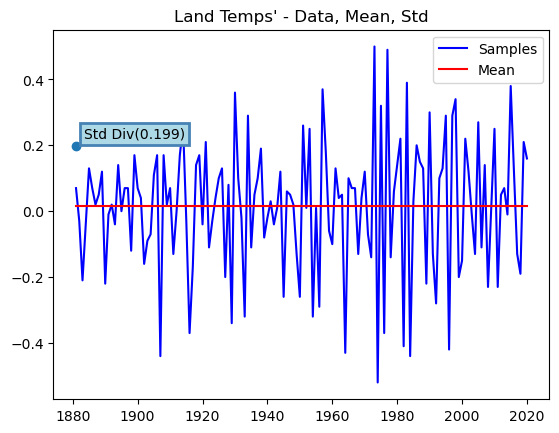
\includegraphics[width=\textwidth]{img/global_temp_dt/data.png}
    \caption{Global Temp $d/dt$ Data}
    \label{fig:global_temp_dtlines}
  \end{subfigure}
  \hfill
  \begin{subfigure}[b]{0.45\textwidth}
    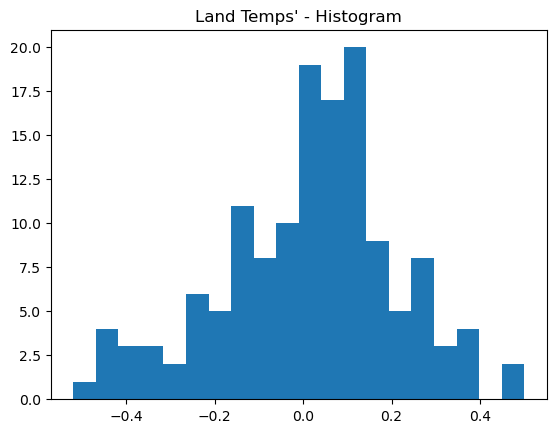
\includegraphics[width=\textwidth]{img/global_temp_dt/histogram.png}
    \caption{Global Temp $d/dt$ Histogram (20 Buckets)}
    \label{fig:global_temp_dthist}
  \end{subfigure}
  \caption{Line and Histogram Plots}
  \label{fig:global_temp_dt1}
\end{figure}
\begin{figure}[htbp]
  \centering
  \begin{subfigure}[b]{0.45\textwidth}
    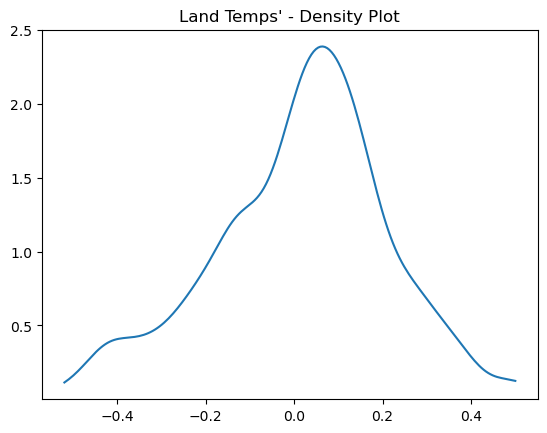
\includegraphics[width=\textwidth]{img/global_temp_dt/density_plot.png}
    \caption{Global Temp $d/dt$ Density Plot}
    \label{fig:global_temp_dtdensity}
  \end{subfigure}
  \hfill
  \begin{subfigure}[b]{0.45\textwidth}
    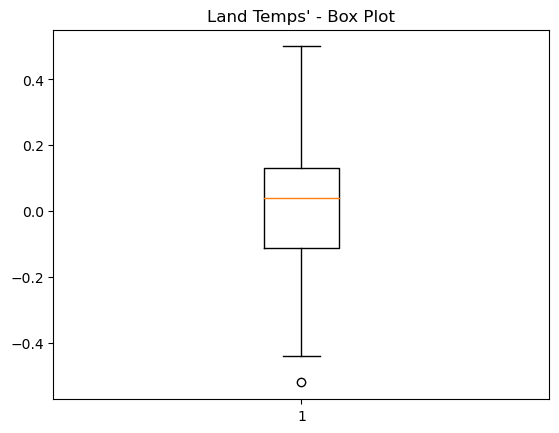
\includegraphics[width=\textwidth]{img/global_temp_dt/box_plot.png}
    \caption{Global Temp $d/dt$ Box Plot}
    \label{fig:global_temp_dtbox}
  \end{subfigure}
  \caption{Density and Box Plot}
  \label{fig:global_temp_dt2}
\end{figure}
\begin{figure}[htbp]
  \centering
  \begin{subfigure}[b]{0.45\textwidth}
    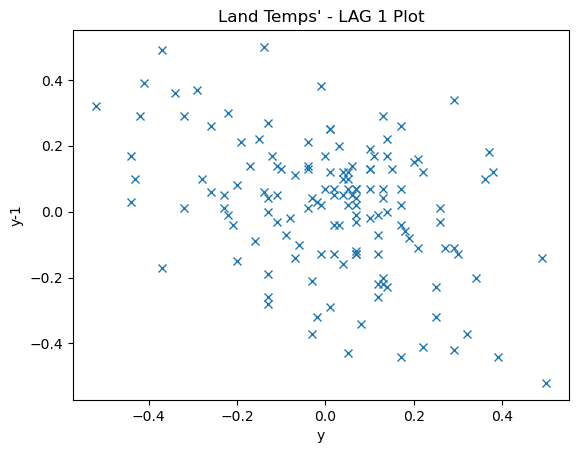
\includegraphics[width=\textwidth]{img/global_temp_dt/lag_1.png}
    \caption{Global Temp $d/dt$ Lag$_1$}
    \label{fig:global_temp_dtlag}
  \end{subfigure}
  \hfill
  \begin{subfigure}[b]{0.45\textwidth}
    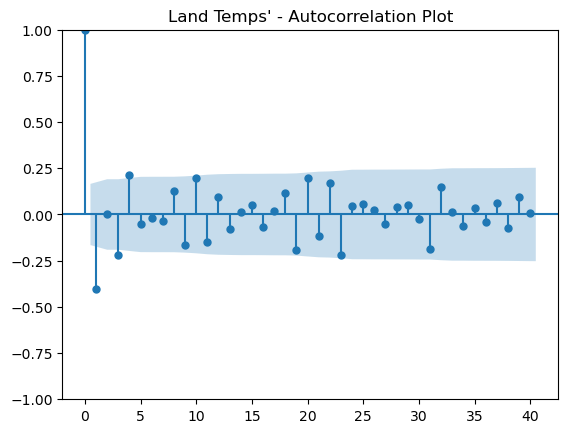
\includegraphics[width=\textwidth]{img/global_temp_dt/acf.png}
    \caption{Global Temp $d/dt$ ACF}
    \label{fig:global_temp_dtacf}
  \end{subfigure}
  \caption{Lag and ACF plots}
  \label{fig:global_temp_dt3}
\end{figure}
\begin{figure}[htbp]
  \centering
  \begin{subfigure}[b]{0.45\textwidth}
    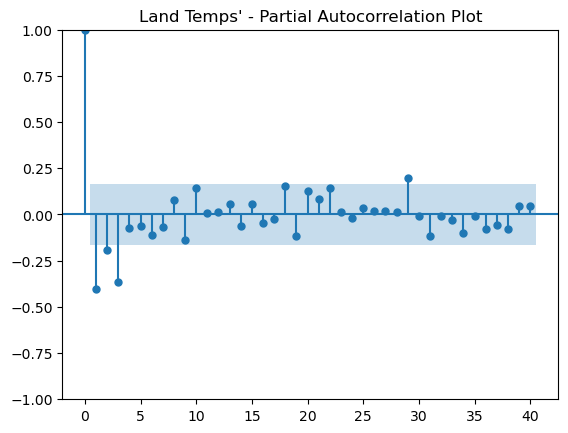
\includegraphics[width=\textwidth]{img/global_temp_dt/pacf.png}
    \caption{Global Temp PACF}
    \label{fig:global_pacf}
  \end{subfigure}
  \hfill
  \begin{subfigure}[b]{0.45\textwidth}
    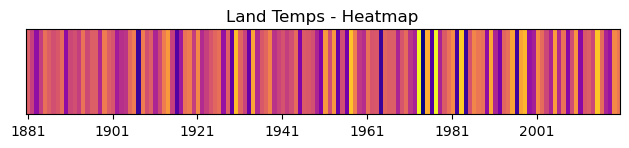
\includegraphics[width=\textwidth]{img/global_temp_dt/heatmap.png}
    \caption{Global Temp Heatmap}
    \label{fig:global_heatmap}
  \end{subfigure}
  \caption{PACF and Heatmap}
  \label{fig:global_temp4}
\end{figure}
 \subsubsection{Test if the original and the differenced temperature anomaly series are random or not.}
 To test the randomness of the series we perform the Ljung-Box test. In the first case we have that the lb\_pvalue is 1.399223e-176 which is much lesser than 0.05 so we can say that the series is not random. In the case of the first order difference we have that the lb\_pvalue is 3.112541e-07 so again we can confirm that the series is not random.
 
 \subsubsection{Test if the original and the differenced temperature anomaly series are stationary or not}
 
 To check for stationary we perform the ADF test, and get an ADF statistic of 0.839 with the critical values being -.479, -2.883 and -2.578 for the fisrt series. The ADF statictic is bigger than the critical values and the p-value is 0.992 which is bigger than 0.05 so we can confirm that the data is not stationary. 
 On the other hand for the second series we have an ASF statistic of -12.216 with the critical values -3.479, -2.883 and -2.578. In this case the ADF statistic is smaller than the critical values and the P-value is 1.133e-22 which is smaller than 0.05 so we can confirm that the series is stationary.
 \subsubsection{Perform the classical decomposition and STL decomposition on the dataset.}
 To do the decompositions in python we use the statsmodels package, specifically the functions seasonaldecompose and STL. A period of 10 was used based on the PACF graph showing a nearly insignificant correlation every 10 years. For the seasonal decompose we choose the additive option. The results are the following:
 
    \begin{figure}[H]
    \centering
    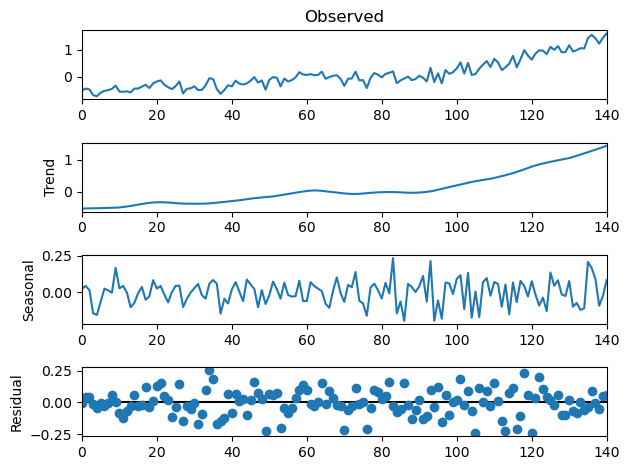
\includegraphics[width=0.4\linewidth]{img/global_temp/seasonal_decomp.png}
    \caption{Global Temp seasonal decomposition}
    \label{fig:global_temp_decomp}
    \end{figure}
    \begin{figure}[H]
    \centering
    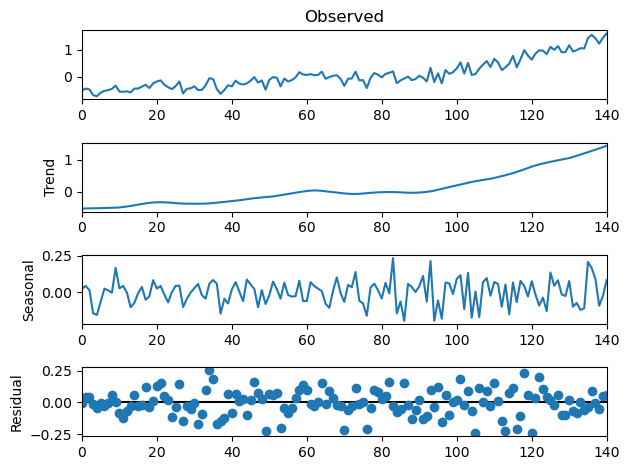
\includegraphics[width=0.4\linewidth]{img/global_temp/stl.png}
    \caption{Global Temp STL}
    \label{fig:global_temp_stl}
    \end{figure}
    
\subsubsection*{ Answer the following questions:}
\begin{itemize}
    \item \textbf{What is a stationary time series?}
\end{itemize}

A stationary time series a collection of data where means and variance are generally constant across time and data.
\begin{itemize}
    \item \textbf{If a series is not stationary, is it possible to transform it into a stationary one? If so, give one technique to do it?}
\end{itemize}

If a series is not stationary partial decomposition can remove some overarching trend data to create a stationary plot.

\begin{itemize}
    \item \textbf{Is the global land temperature anomaly series stationary? Why or why not?}
\end{itemize}

The global land temperature anomaly series is not stationary, because it fails the ADF test and has a visual upwards trend.

\begin{itemize}
    \item \textbf{Is the data set after the first-order difference stationary?}
\end{itemize}
Yes after the first order differentiation the data is stationary according to ADF.
\begin{itemize}
    \item \textbf{Why is it useful to decompose a time series into a few components? What are the typical component in a time series decomposition?}
\end{itemize}
Splitting a time series into multiple components makes it easier to take advantage of individual models strengths. For example with seasonal decomposition used in this lab are split into trend, seasonal and residual models. The trend covers over arching changes, when seasonal models period data, and then the residual should be white noise to represent uncorrelated data.


\section{Task 2. Feature Extraction}

\subsection{Task 2.1. Frequency components of a synthetic time-series signal}
\subsubsection{ Draw a line plot of the series.}

To generate a series of five sequential sine wave signals we will use the following code:

\begin{listing}[!ht]
\begin{minted}{python}

total_duration = 5  # Total duration of the signal in seconds
sampling_rate = 200  # Sampling rate in Hz
t = np.linspace(0, total_duration, total_duration * sampling_rate, endpoint=False)

frequencies = [10, 20, 30, 40, 50]  # Frequencies in Hz for each second
signal = np.zeros_like(t)
for i, freq in enumerate(frequencies, 1):
    mask = (t >= i - 1) & (t < i)  # Mask for each second
    signal[mask] = np.sin(2 * np.pi * freq * t[mask])
  
\end{minted}
\caption{Sine waves Series Generator}
\label{listing:gen_sin}
\end{listing}
Which creates a series of five different sine signals with frequency changing frequencies and duration 1 second. Once the signals is generated we can obtain its line plot.
 \begin{figure}
    \centering 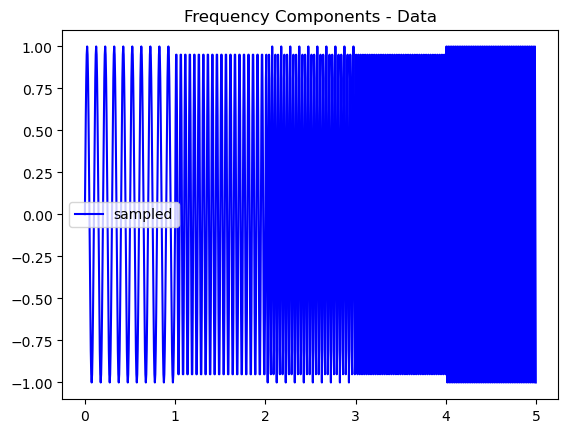
\includegraphics[width=0.6\linewidth]{img/stacked_sin/data.png}
    \caption{Sine waves series line plot}
    \label{fig:sine_waves_line}
    \end{figure}
\subsubsection{Draw power spectrum (power density graph) of the series.}
The power sprectrum for the sine waves series has the following form:
    \begin{figure}[H]
    \centering 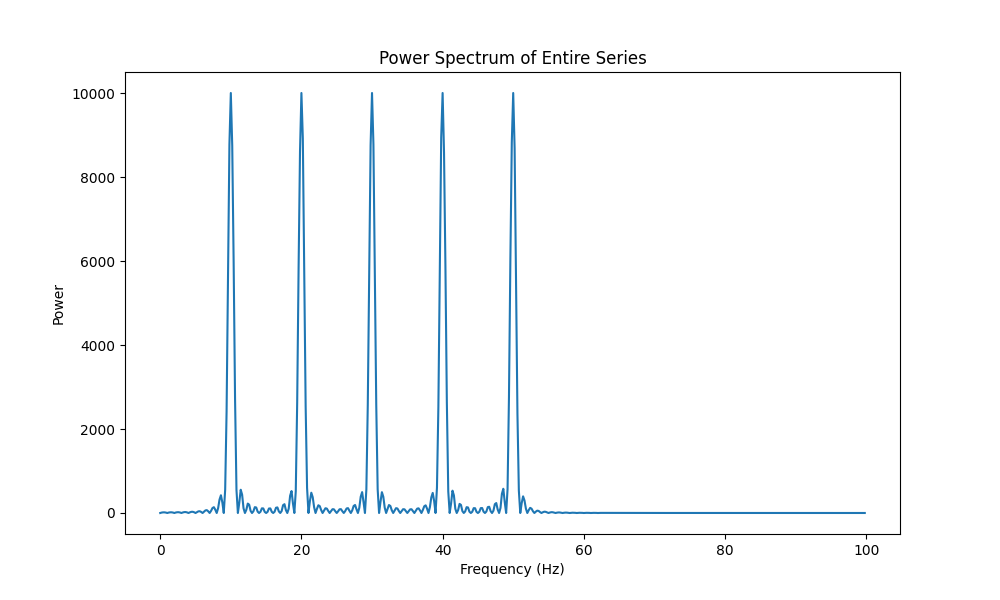
\includegraphics[width=0.6\linewidth]{img/stacked_sin/sines_powerspectrum.png}
    \caption{Sine waves series power spectrum}
    \label{fig:sine_waves_power_spectrum}
    \end{figure}
\subsubsection{Draw the spectrogram of the series.}
The spectogram of the series has the following form:
 \begin{figure}[H]
    \centering 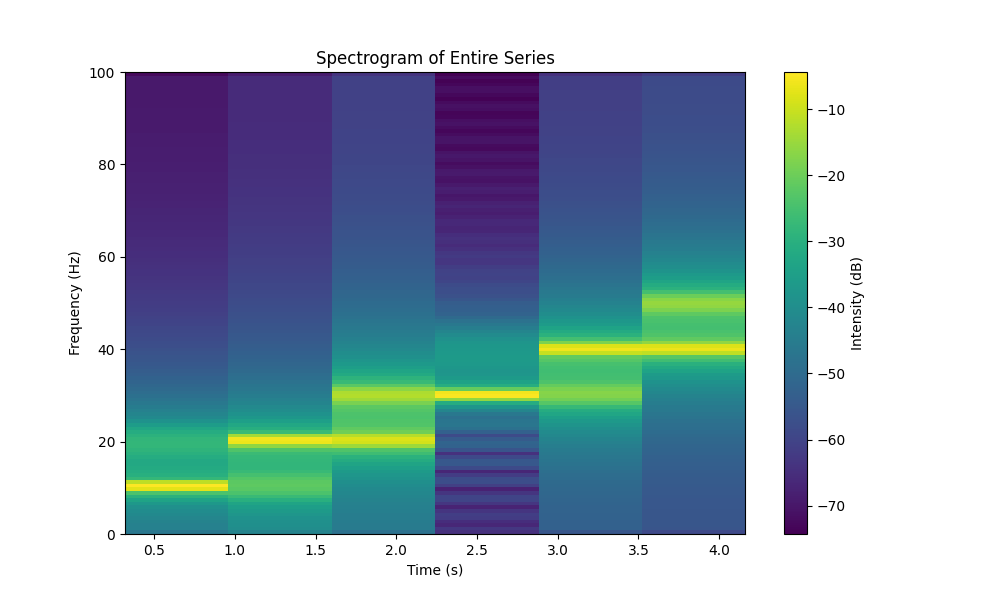
\includegraphics[width=0.6\linewidth]{img/stacked_sin/sines_spectrogram.png}
    \caption{Sine waves series spectogram}
    \label{fig:sine_waves_spectogram}
    \end{figure}
\subsubsection{Draw and compare the ACF and PACF graphs of the first one-second (frequency
 10Hz) and the second one-second series (frequency 20Hz), with lags up to 50.}
By using the already mentiones function we can obtain the ACF and PACF graphs for the furst and second sine waves. 
\begin{figure}[htbp]
  \centering
  \begin{subfigure}[b]{0.45\textwidth}
    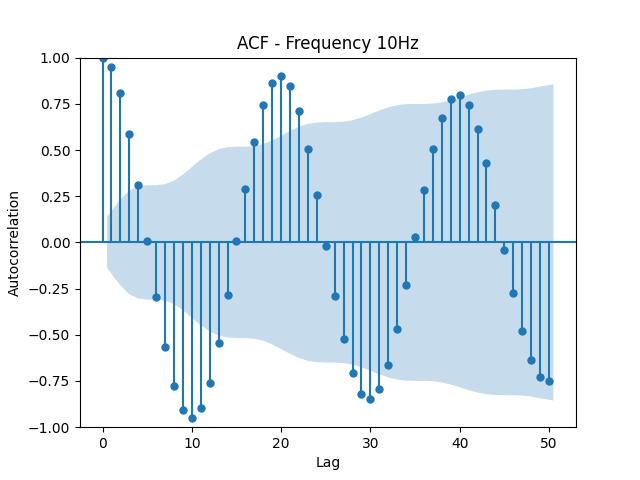
\includegraphics[width=\textwidth]{img/stacked_sin/ACF10HZ.png}
    \caption{ACF for 10 Hz sine signal}
    \label{fig:acf10}
  \end{subfigure}
  \hfill
  \begin{subfigure}[b]{0.45\textwidth}
    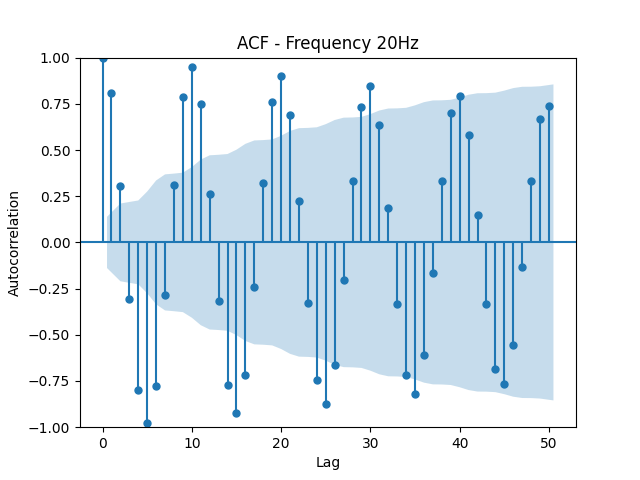
\includegraphics[width=\textwidth]{img/stacked_sin/ACF20HZ.png}
    \caption{ACF for 20 Hz sine signal}
    \label{fig:acf20}
  \end{subfigure}
  \caption{ACF plots}
  \label{fig:ACFsines}
\end{figure}
\begin{figure}[htbp]
  \centering
  \begin{subfigure}[b]{0.45\textwidth}
    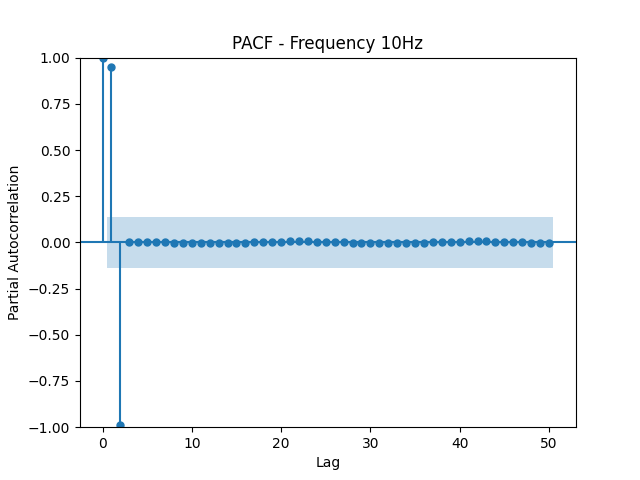
\includegraphics[width=\textwidth]{img/stacked_sin/PACF10HZ.png}
    \caption{PACF for 10 Hz sine signal}
    \label{fig:Pacf10}
  \end{subfigure}
  \hfill
  \begin{subfigure}[b]{0.45\textwidth}
    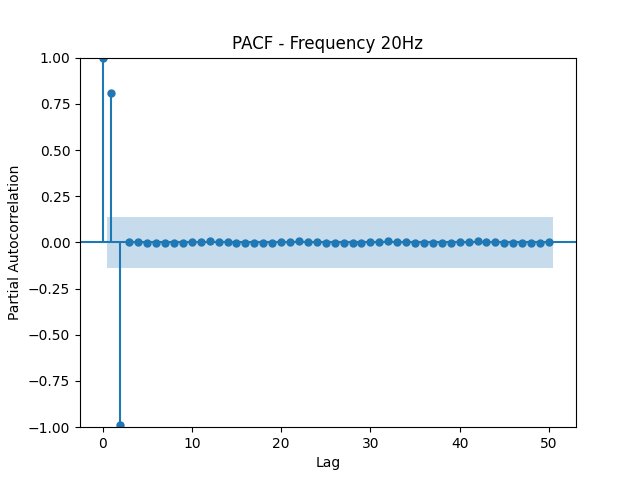
\includegraphics[width=\textwidth]{img/stacked_sin/PACF20HZ.png}
    \caption{PACF for 20 Hz sine signal}
    \label{fig:pacf20}
  \end{subfigure}
  \caption{PACF plots}
  \label{fig:ACFsines}
\end{figure}
\subsection{Task 2.2. Statistical features and discovery of event-related potential}
\subsubsection{Visualize the response, i.e., ERP of the EEG, in the two conditions, A and B.}

To extract and manipulate the data we use the provided code and dataset. And then compute the mean of the different experiments to get the ERP for each condition.
\begin{listing}[!ht]
\begin{minted}{python}
 from scipy.io import loadmat
 # Import function to read data.
 data = loadmat('matfiles/02_EEG-1.mat')
 data.keys()
 EEGa = data['EEGa']
 EEGb = data['EEGb']
 t = data['t'][0]
\end{minted}
\caption{Code for extracting ECG data with A and B conditions}
\label{listing:ecg1}
\end{listing}

\begin{figure}[H]
    \centering 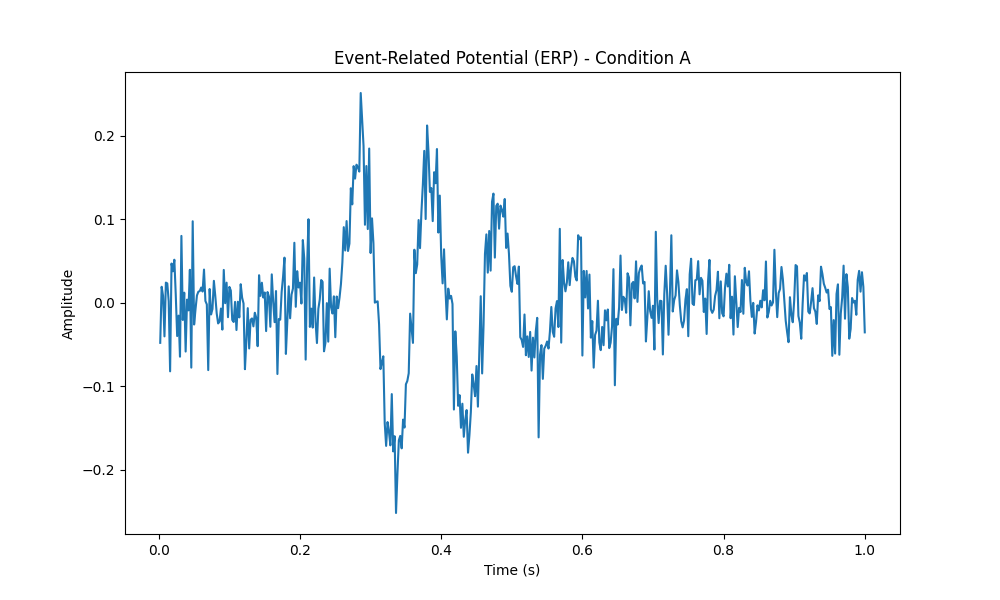
\includegraphics[width=0.6\linewidth]{img/ecg1/ECGA.png}
    \caption{ERP for condition A}
    \label{fig:erpA}
    \end{figure}
\begin{figure}[H]
    \centering 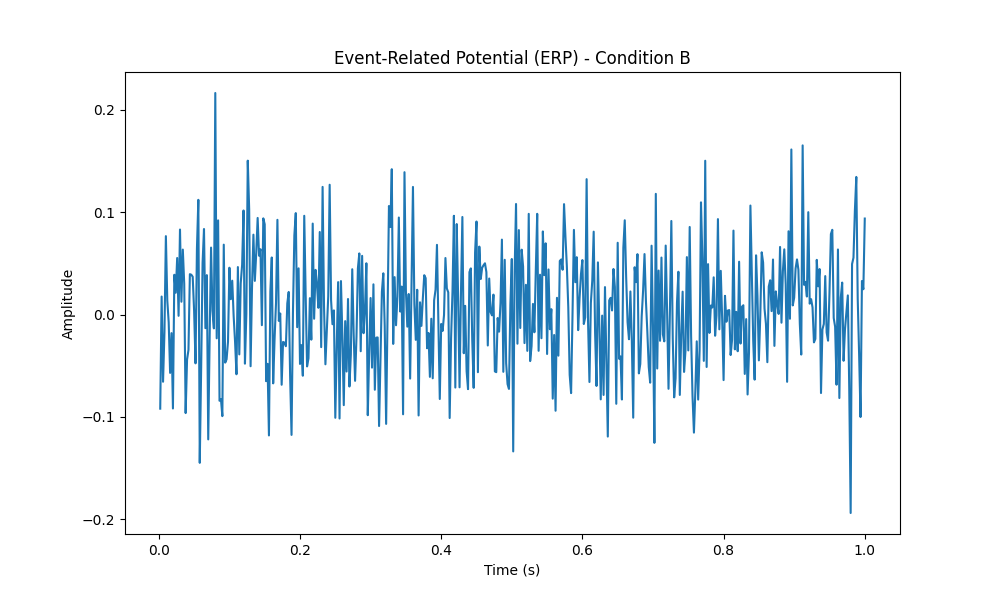
\includegraphics[width=0.6\linewidth]{img/ecg1/ECGB.png}
    \caption{ERP for condition B}
    \label{fig:erpB}
    \end{figure}    
\subsubsection{Find the brain activity frequency in the data of condition A (see below for condition
 A and B).}

 To find the brain activity frequency we will use the season decomposition as in the previous sections, achieving the following results.
 \begin{figure}[H]
    \centering 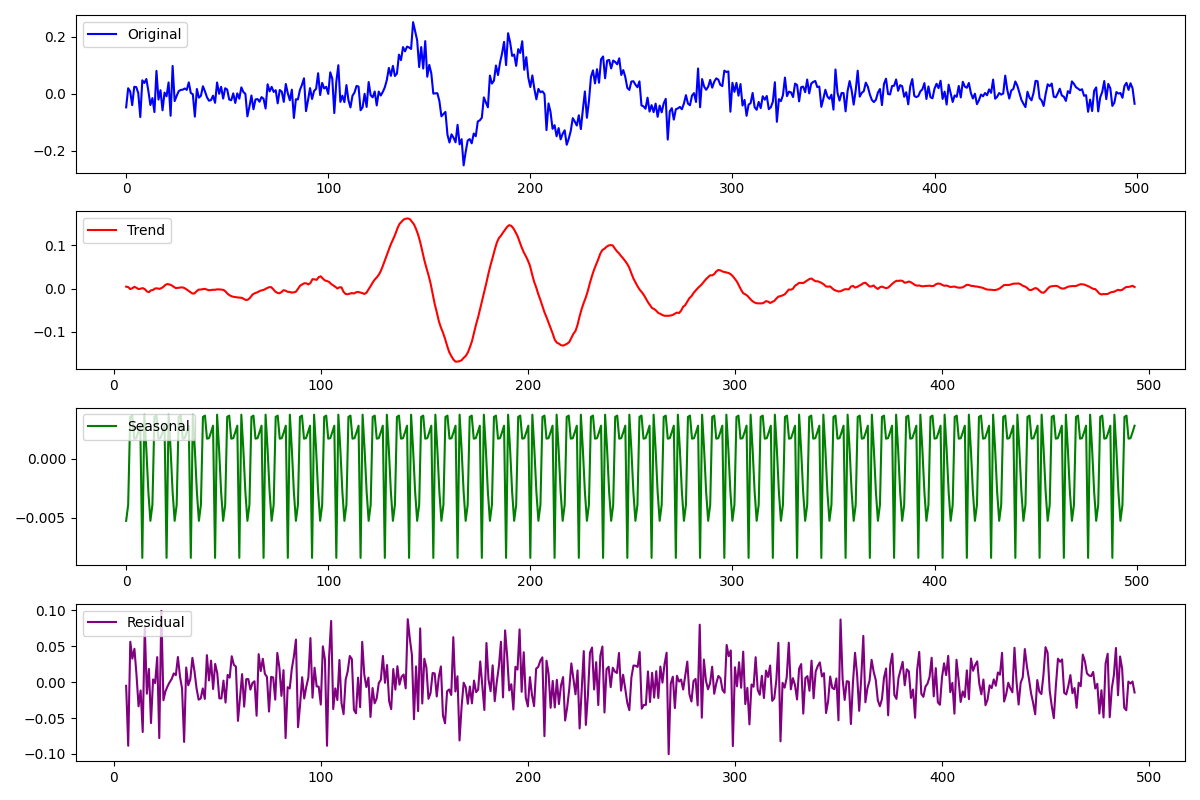
\includegraphics[width=0.6\linewidth]{img/ecg1/Erpa_seasonaldecomposition.png}
    \caption{Seasonal decomposition for ERP for condition A}
    \label{fig:erpA_decomposed}
    \end{figure}  
 
\subsection{Task 2.3. Features of observed rhythms in EEG}

\subsubsection{For the EEG data set, draw the line plot, histogram, density plot, box plot, lag-1
 plot, ACF and PACF graphs (lags up to 50)}
 The plots are computed as the previous ones:
 
 \begin{figure}[htbp]
  \centering
  \begin{subfigure}[b]{0.45\textwidth}
    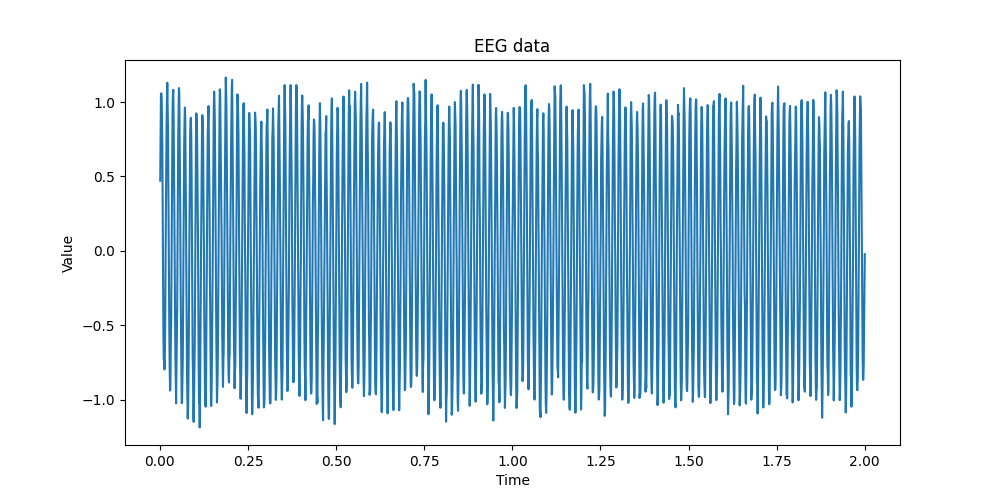
\includegraphics[width=\textwidth]{img/ecg2/ECGlineplot.png}
    \caption{ECG signal}
    \label{fig:ecg_line}
  \end{subfigure}
  \hfill
  \begin{subfigure}[b]{0.45\textwidth}
    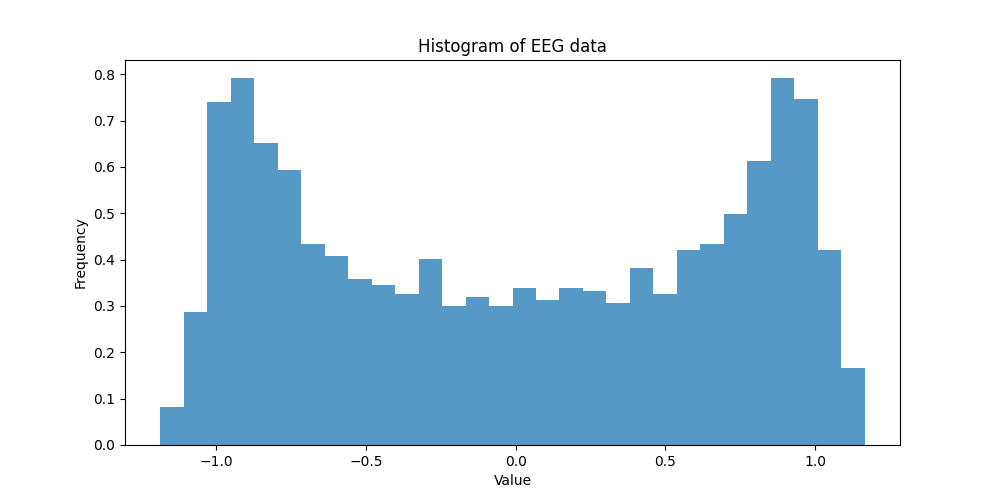
\includegraphics[width=\textwidth]{img/ecg2/ECGhistogram.png}
    \caption{ECG Histogram (20 Buckets)}
    \label{fig:ecghist}
  \end{subfigure}
  \caption{Line and Histogram Plots}
  \label{fig:ecg2_1}
\end{figure}
\begin{figure}[htbp]
  \centering
  \begin{subfigure}[b]{0.45\textwidth}
    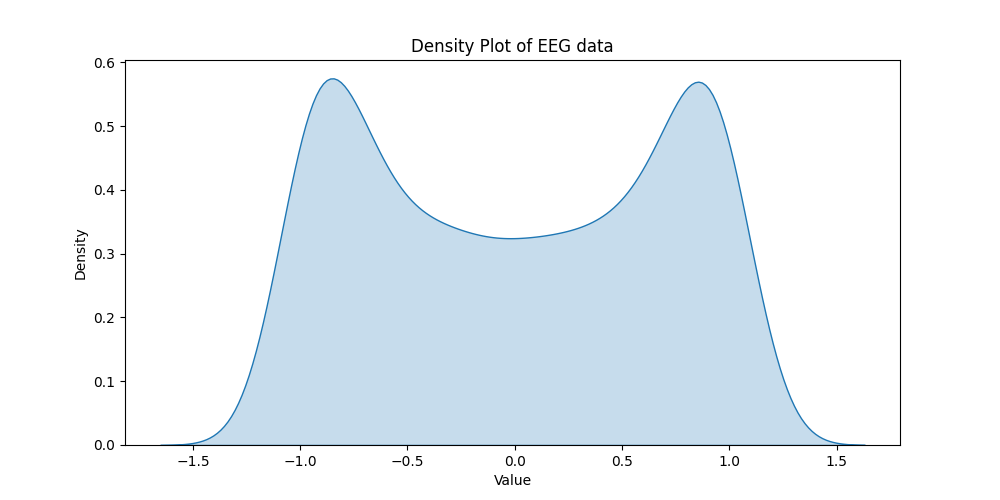
\includegraphics[width=\textwidth]{img/ecg2/ECGdensity.png}
    \caption{ECG Density Plot}
    \label{fig:ecgdensity}
  \end{subfigure}
  \hfill
  \begin{subfigure}[b]{0.45\textwidth}
    \includegraphics[width=\textwidth]{img/ecg2/ECGbox.png}
    \caption{ECG Box Plot}
    \label{fig:ecgbox}
  \end{subfigure}
  \caption{Density and Box Plot}
  \label{fig:ecg2_2}
\end{figure}
\begin{figure}[htbp]
  \centering
  \begin{subfigure}[b]{0.45\textwidth}
    \includegraphics[width=\textwidth]{img/ecg2/ECGlag.png}
    \caption{ECG Lag$_1$}
    \label{fig:ecglag}
  \end{subfigure}
  \hfill
  \begin{subfigure}[b]{0.45\textwidth}
    \includegraphics[width=\textwidth]{img/ecg2/ECGacf.png}
    \caption{ECG ACF}
    \label{fig:ecgacf}
  \end{subfigure}
  \caption{Lag and ACF plots}
  \label{fig:global_temp_dt3}
\end{figure}
\begin{figure}
    \centering \includegraphics[width=0.7\linewidth]{img/ecg2/ECGlpacf.png}
    \caption{ECG for PACF}
    \label{fig:ecgpacf}
    \end{figure}

\subsubsection{ Show the statistical characteristics of the EEG data, such as mean, variance, standard deviation}
By using the functions in the package numpy we can get the following results:
\begin{itemize}
    \item Mean of EEG Data: 2.73e-17
    \item Variance of EEG Data: 0.50
    \item Standard Deviation of EEG Data: 0.71
\end{itemize}


\subsubsection{Compute the auto-covariance of the EEG data. Draw and save the auto-covariance graph. Examine the auto-covariance plot, Why does the auto-covariance exhibit repeated peaks and troughs approximately every 0.0166 s?}

In Figure \ref{fig:ecgcovariance} we can see the auto-covariance graph.
 \begin{figure}[H]
    \centering \includegraphics[width=0.7\linewidth]{img/ecg2/auto_covariance_plot.png}
    \caption{Auto covariance of ECG plot}
    \label{fig:ecgcovariance}
    \end{figure}
We can see repeated peaks and troughs at 0.0166s because there is an underlying oscillations that repeats itself in that time period. That means that the oscillation has a frequency of $1/f = 60Hz$
\subsubsection{ Compute and plot the power-spectrum of the EEG data. Show it in both linear scale
 and log (dB) scale. To emphasize low-amplitude rhythms hidden by large-amplitude
 oscillations is to change the scale of the spectrum to decibels.}
In Figure \ref{fig:ecgpower_spectrumlinear} we can see the power spectrum in linear units and in Figure \ref{fig:ecgpower_spectrumlog} we can see the graph with logarithmic units.
  \begin{figure}[H]
    \centering \includegraphics[width=0.7\linewidth]{img/ecg2/power_spectrum_linear.png}
    \caption{Power spectrum of ECG with linear units}
    \label{fig:ecgpower_spectrumlinear}
    \end{figure}
     \begin{figure}[H]
    \centering \includegraphics[width=0.7\linewidth]{img/ecg2/power_spectrum_log.png}
    \caption{Power spectrum of ECG with logarithmic units}
    \label{fig:ecgpower_spectrumlog}
    \end{figure}
\subsubsection*{Now it is
 time to answer the following questions:}
 \begin{itemize}
     \item \textbf{What features do you typically consider useful for analyzing and modeling time series data?}
     
     
     There are several features, as we have seen throughout this exercise, that can be useful for analyzing and modeling time series, such as statistical features like mean, variance, standard deviation etc. Temporal features like the autocorrelation, autocovariance, the periodicity or the stationarity, and also frequency domain features like the power spectral density.
 \end{itemize}
  \begin{itemize}
     \item \textbf{What features are specific for time-series, and what are general for both time-series and non-time-series data?}
     
     
     The features that are specific for time series are those related to the time variable of the series such as the autocorrelation, autocovariance, periodicity and stationarity. The rest of the features can be shared both by time and non-time series.
 \end{itemize}
  \begin{itemize}
     \item \textbf{How are auto-covariance and auto-correlation are defined for a time series? Give mathematical formulas for the definitions.}
     
     
     The auto-covariance measures the linear dependence between two observations in a time series separated by a specific lag. The formula to calculate it is:
      \end{itemize}

      
    \begin{equation}
        r_{xx}[L] = \frac{1}{N}\sum_{n=1}^{N - L} (x_{n+L} - \overline{x})(x_{n} - \overline{x})
    \end{equation}

    

The auto-correlation normalizes the auto-covariance to have values between -1 and 1 indicating the strength and direction at a linear relationship at a given lag. The formula to calculate it is:


\begin{equation}
        \rho_{xx}[L] = \frac{r_{xx}[L]}{\sigma^2}
    \end{equation}

    

  \begin{itemize}
     \item \textbf{Assume a short time-series {1,2,3,4,5,6,7,8,7,6,5,4,3,2,1}. (1) Calculate the auto-covariance and auto-correlations for all valid lags. Do the calculations manually. (2) Write a Python program to validate your calculations. (3) Draw the ACF graph for the time series}
 \end{itemize}

 We will use the formula described in the previous section to compute the auto-covariance and the auto-correlation. In the first place we calculate the mean as:
 \begin{equation}
     \overline{x} = \frac{\sum{x_i}}{N} = 4.26
 \end{equation}
 With this value we can calculate  the auto-covariance and auto-correlation at each valid lag as.

 
 We have for L = 15
 \begin{equation}
      r_{xx}[L] = \frac{1}{N}\sum_{n=1}^{N - L} (x_{n+L} - \overline{x})(x_{n} - \overline{x}) = 0.066
      %\frac{1}{15} = 0.066
 \end{equation}
 For L = 14
 \begin{equation}
      r_{xx}[L] = \frac{1}{N}\sum_{n=1}^{N - L} (x_{n+L} - \overline{x})(x_{n} - \overline{x}) = 0.708
      %\frac{1}{15}(1 - 4.26)(1 - 4.26) = 0.708
 \end{equation}
 For L = 13
 \begin{equation}
      r_{xx}[L] = \frac{1}{N}\sum_{n=1}^{N - L} (x_{n+L} - \overline{x})(x_{n} - \overline{x}) = 0.982
      %\frac{1}{15}[(2 - 4.26)(1 - 4.26) + (2 - 4.26)(1 - 4.26)] = 0.982
 \end{equation}
  For L = 12
 \begin{equation}
      r_{xx}[L] = \frac{1}{N}\sum_{n=1}^{N - L} (x_{n+L} - \overline{x})(x_{n} - \overline{x}) =  0.888
      %\frac{1}{15}[(3 - 4.26)(1 - 4.26) + (2 - 4.26)(2 - 4.26) + (1 - 4.26)(3 - 4.26)] = 0.888
 \end{equation}
  For L = 11
 \begin{equation}
      r_{xx}[L] = \frac{1}{N}\sum_{n=1}^{N - L} (x_{n+L} - \overline{x})(x_{n} - \overline{x}) = 0.492
      %\frac{1}{15}[(4 - 4.26)(1 - 4.26) + (3 - 4.26)(2 - 4.26) + (2 - 4.26)(3 - 4.26) + (1 - 4.26)(4 - 4.26)] = 0.492
 \end{equation}
 For L = 10
  \begin{equation}
      r_{xx}[L] = \frac{1}{N}\sum_{n=1}^{N - L} (x_{n+L} - \overline{x})(x_{n} - \overline{x}) = -0.137
      %\frac{1}{15}[(5 - 4.26)(1 - 4.26) + (4 - 4.26)(2 - 4.26) + (3 - 4.26)(3 - 4.26) + (2 - 4.26)(4 - 4.26) + (1 - 4.26)(5 - 4.26)] = -0.137
 \end{equation}
  For L = 9
  \begin{equation}
      r_{xx}[L] = \frac{1}{N}\sum_{n=1}^{N - L} (x_{n+L} - \overline{x})(x_{n} - \overline{x}) = -0.935
      %\frac{1}{15}[(6 - 4.26)(1 - 4.26) + (5 - 4.26)(2 - 4.26) + (4 - 4.26)(3 - 4.26) + (3 - 4.26)(4 - 4.26) + (2 - 4.26)(5 - 4.26)  + (1 - 4.26)(6 - 4.26)] = -0.935
 \end{equation}
  For L = 8
  \begin{equation}
      r_{xx}[L] = \frac{1}{N}\sum_{n=1}^{N - L} (x_{n+L} - \overline{x})(x_{n} - \overline{x}) = -1.835
      %\frac{1}{15}[(7 - 4.26)(1 - 4.26) + (6 - 4.26)(2 - 4.26) + (5 - 4.26)(3 - 4.26) + (4 - 4.26)(4 - 4.26) + (3 - 4.26)(5 - 4.26) + (2 - 4.26)(6 - 4.26)  + (1 - 4.26)(7 - 4.26)] = -1.835
 \end{equation}
  For L = 7
  \begin{equation}
      r_{xx}[L] = \frac{1}{N}\sum_{n=1}^{N - L} (x_{n+L} - \overline{x})(x_{n} - \overline{x}) = -2.666
      %\frac{1}{15}[(8 - 4)(1 - 4) + (7 - 4)(2 - 4) +(6 - 4)(3 - 4) + (5 - 4)(4 - 4) + (4 - 4)(5 - 4) + (3 - 4)(6 - 4) + (2 - 4)(7 - 4)  + (1 - 4)(8 - 4)] = -2.666
 \end{equation}
  For L = 6
  \begin{equation}
      r_{xx}[L] = \frac{1}{N}\sum_{n=1}^{N - L} (x_{n+L} - \overline{x})(x_{n} - \overline{x}) = -2.6
      %\frac{1}{15}[(7 - 4)(1 - 4) +(8 - 4)(2 - 4) + (7 - 4)(3 - 4) +(6 - 4)(4 - 4) + (5 - 4)(5 - 4) + (4 - 4)(6 - 4) + (3 - 4)(7 - 4) + (2 - 4)(8 - 4)  + (1 - 4)(7 - 4)] = -2.6
 \end{equation}
   For L = 5
  \begin{equation}
      r_{xx}[L] = \frac{1}{N}\sum_{n=1}^{N - L} (x_{n+L} - \overline{x})(x_{n} - \overline{x}) = -1.866
      %\frac{1}{15}[(6 - 4)(1 - 4) + (7 - 4)(2 - 4) +(8 - 4)(3 - 4) + (7 - 4)(4 - 4) +(6 - 4)(5 - 4) + (5 - 4)(6 - 4) + (4 - 4)(7 - 4) + (3 - 4)(8 - 4) + (2 - 4)(7 - 4)  + (1 - 4)(6 - 4)] = -1.866
 \end{equation}
   For L = 4
  \begin{equation}
      r_{xx}[L] = \frac{1}{N}\sum_{n=1}^{N - L} (x_{n+L} - \overline{x})(x_{n} - \overline{x}) = -0.666
      %\frac{1}{15}[(5 - 4)(1 - 4) + (6 - 4)(2 - 4) + (7 - 4)(3 - 4) +(8 - 4)(4 - 4) + (7 - 4)(5 - 4) +(6 - 4)(6 - 4) + (5 - 4)(7 - 4) + (4 - 4)(8 - 4) + (3 - 4)(7 - 4) + (2 - 4)(6 - 4)  + (1 - 4)(5 - 4)] = -0.666
 \end{equation}
   For L = 3
  \begin{equation}
      r_{xx}[L] = \frac{1}{N}\sum_{n=1}^{N - L} (x_{n+L} - \overline{x})(x_{n} - \overline{x}) = 0.8
      %\frac{1}{15}[(4 - 4)(1 - 4) + (5 - 4)(2 - 4) + (6 - 4)(3 - 4) + (7 - 4)(4 - 4) +(8 - 4)(5 - 4) + (7 - 4)(6 - 4) +(6 - 4)(7 - 4) + (5 - 4)(8 - 4) + (4 - 4)(7 - 4) + (3 - 4)(6 - 4) + (2 - 4)(5 - 4)  + (1 - 4)(4 - 4)] = 0.8
 \end{equation}
   For L = 2
  \begin{equation}
      r_{xx}[L] = \frac{1}{N}\sum_{n=1}^{N - L} (x_{n+L} - \overline{x})(x_{n} - \overline{x}) = 2.33
      %\frac{1}{15}[(3 - 4)(1 - 4) + (4 - 4)(2 - 4) + (5 - 4)(3 - 4) + (6 - 4)(4 - 4) + (7 - 4)(5 - 4) +(8 - 4)(6 - 4) + (7 - 4)(7 - 4) +(6 - 4)(8 - 4) + (5 - 4)(7 - 4) + (4 - 4)(6 - 4) + (3 - 4)(5 - 4) + (2 - 4)(4 - 4)  + (1 - 4)(3 - 4)] = 2.33
 \end{equation}
   For L = 1
  \begin{equation}
      r_{xx}[L] = \frac{1}{N}\sum_{n=1}^{N - L} (x_{n+L} - \overline{x})(x_{n} - \overline{x}) = 3.73
      %\frac{1}{15}[(2 - 4)(1 - 4) + (3 - 4)(2 - 4) + (4 - 4)(3 - 4) + (5 - 4)(4 - 4) + (6 - 4)(5 - 4) + (7 - 4)(6 - 4) +(8 - 4)(7 - 4) + (7 - 4)(8 - 4) +(6 - 4)(7 - 4) + (5 - 4)(6 - 4) + (4 - 4)(5 - 4) + (3 - 4)(4 - 4) + (2 - 4)(3 - 4)  + (1 - 4)(2 - 4)] = 3.73
 \end{equation}
   For L = 0
  \begin{equation}
      r_{xx}[L] = \frac{1}{N}\sum_{n=1}^{N - L} (x_{n+L} - \overline{x})(x_{n} - \overline{x}) = 4.8
      %\frac{1}{15}[(1 - 4)(1 - 4) + (2 - 4)(2 - 4) + (3 - 4)(3 - 4) + (4 - 4)(4 - 4) + (5 - 4)(5 - 4) + (6 - 4)(6 - 4) + (7 - 4)(7 - 4) +(8 - 4)(8 - 4) + (7 - 4)(7 - 4) +(6 - 4)(6 - 4) + (5 - 4)(5 - 4) + (4 - 4)(4 - 4) + (3 - 4)(3 - 4) + (2 - 4)(2 - 4)  + (1 - 4)(1 - 4)] = 4.8
 \end{equation}
 To calculate the auto correlation at each lag first we calculate the variance as :
   \begin{equation}
      \sigma^2 = \frac{1}{N}\sum_{n=1}^{N} (x_{n} - \overline{x})^2 = 4.72
 \end{equation}

 An then we can calculate the auto-correlation at each lag:

 
We have for L = 15
 \begin{equation}
       \rho_{xx}[L] = \frac{r_{xx}[L]}{\sigma ^2} = \frac{0.066}{22.36} = 0.003
 \end{equation}
 For L = 14
 \begin{equation}
       \rho_{xx}[L] = \frac{r_{xx}[L]}{\sigma ^2} = \frac{0.708}{22.36} = 0.032
 \end{equation}
 For L = 13
 \begin{equation}
       \rho_{xx}[L] = \frac{r_{xx}[L]}{\sigma ^2} = \frac{0.982}{22.36} = 0.044
 \end{equation}
  For L = 12
 \begin{equation}
       \rho_{xx}[L] = \frac{r_{xx}[L]}{\sigma ^2} = \frac{0.888}{22.36} = 0.039
 \end{equation}
  For L = 11
 \begin{equation}
       \rho_{xx}[L] = \frac{r_{xx}[L]}{\sigma ^2} = \frac{0.492}{22.36} = 0.022
 \end{equation}
 For L = 10
  \begin{equation}
       \rho_{xx}[L] = \frac{r_{xx}[L]}{\sigma ^2} = \frac{-0.137}{22.36} = -0.006
 \end{equation}
  For L = 9
  \begin{equation}
       \rho_{xx}[L] = \frac{r_{xx}[L]}{\sigma ^2} = \frac{-0.935}{22.36} = -0.41
 \end{equation}
  For L = 8
  \begin{equation}
       \rho_{xx}[L] = \frac{r_{xx}[L]}{\sigma ^2} = \frac{-1.835}{22.36} = -0.08
 \end{equation}
  For L = 7
  \begin{equation}
       \rho_{xx}[L] = \frac{r_{xx}[L]}{\sigma ^2} = \frac{-2.666}{22.36} = -0.11
 \end{equation}
  For L = 6
  \begin{equation}
       \rho_{xx}[L] = \frac{r_{xx}[L]}{\sigma ^2} = \frac{-2.6}{22.36} = -0.11
       \end{equation}
   For L = 5
  \begin{equation}
       \rho_{xx}[L] = \frac{r_{xx}[L]}{\sigma ^2} = \frac{-1.866}{22.36} = -0.08
 \end{equation}
   For L = 4
  \begin{equation}
        \rho_{xx}[L] = \frac{r_{xx}[L]}{\sigma ^2} = \frac{-0.666}{22.36} = -0.02
 \end{equation}
   For L = 3
  \begin{equation}
       \rho_{xx}[L] = \frac{r_{xx}[L]}{\sigma ^2} = \frac{0.8}{22.36} = 0.03
 \end{equation}
   For L = 2
  \begin{equation}
       \rho_{xx}[L] = \frac{r_{xx}[L]}{\sigma ^2} = \frac{2.33}{22.36} = 0.10
 \end{equation}
   For L = 1
  \begin{equation}
       \rho_{xx}[L] = \frac{r_{xx}[L]}{\sigma ^2} = \frac{3.73}{22.36} = 0.16
 \end{equation}
   For L = 0
  \begin{equation}
      \rho_{xx}[L] = \frac{r_{xx}[L]}{\sigma ^2} = \frac{4.8}{22.36} = 0.21
 \end{equation}
To compute the auto-covariance and auto-correlation in Python we yse the following code:

\begin{listing}[H]
\begin{minted}{python}

x = np.array([1, 2, 3, 4, 5, 6, 7, 8, 7, 6, 5, 4, 3, 2, 1])
mean = np.mean(x)
variance = np.var(x)
N = 15
sum_covariance = 0
auto_covariance = []
auto_correlation = []
for l in range(14,-1,-1):
    sum_covariance = 0
    for n in range(N - l):
        sum_covariance += (x[n + l] - mean) * (x[n] - mean)

    auto_covariance.append((1 / N) * sum_covariance)
    auto_correlation.append(((1 / N) * sum_covariance)/(variance*variance))
\end{minted}
\caption{Code for extracting ECG data with A and B conditions}
\label{listing:ecg1}
\end{listing}
 Finally, we compute the ACF graph and get the following result:
 \begin{figure}[H]
    \centering \includegraphics[width=0.7\linewidth]{img/last_task/acf_x.png}
    \caption{ACF for the given time series}
    \label{fig:acf_x}
    \end{figure}


\end{document}
